\documentclass[a4paper]{report}
\usepackage[utf8]{inputenc}
\usepackage[portuguese]{babel}
\usepackage{hyperref}
\usepackage{a4wide}
\hypersetup{pdftitle={Trabalho 1},
pdfauthor={João Teixeira, José Ferreira, Miguel Solino},
colorlinks=true,
urlcolor=blue,
linkcolor=black}
\usepackage{subcaption}
\usepackage[cache=false]{minted}
\usepackage{listings}
\usepackage{booktabs}
\usepackage{multirow}
\usepackage{appendix}
\usepackage{tikz}
\usepackage{authblk}
\usepackage{bashful}
\usepackage{verbatim}
\usepackage{amsmath}
\usetikzlibrary{positioning,automata,decorations.markings}

\begin{document}

\title{Trabalho 1\\ 
\large Grupo Nº 3}
\author{João Teixeira (A85504) \and José Ferreira (A83683) \and Miguel Solino (A86435)}
\date{\today}

\begin{center}
    \begin{minipage}{0.75\linewidth}
        \centering
        
\includegraphics[width=0.4\textwidth]{images/eng.jpeg}\par\vspace{1cm}
        \vspace{1.5cm}
        \href{https://www.uminho.pt/PT}
        {\color{black}{\scshape\LARGE Universidade do Minho}} \par
        \vspace{1cm}
        \href{https://www.di.uminho.pt/}
        {\color{black}{\scshape\Large Departamento de Informática}} \par
        \vspace{1.5cm}
        \maketitle
    \end{minipage}
\end{center}

\tableofcontents

\pagebreak

\chapter{Introdução}
Um dos prblemas \textit{NP-Completo} mais conhecido é o problema do
Caixeiro viajante (\textit{Travelling Salesman Problem}). \\
Quando transferido para um grafo orientado, este problema resume-se
encontrar o caminho mais curto que visite todos os nodos do grafo.\\
Outro problema derivado do problema do Caixeiro Viajante é o problema
do carteiro chinês (\textit{Chinese Postman Problem}). Neste, a única
diferença é que em vez de ser a caminho mais curto que visite todos
os nodos, é o caminho mais curto que visite todas as arestas do grafo. \\
Assim, o objetivo deste trabalho prático é resolver este problema
utilizando programação linear.

\chapter{Problema}
Observando os números de inscrição dos membros do grupo, constatamos
que o maior pertencia ao aluno Miguel Solino (86435).
Fazendo \textit{pattern matching} para o padrão ABCDE e seguindo as
regras definidas no enunciado, concluímos que a orientação das ruas é:

\begin{enumerate}
    \item A é igual a 8;
    \item B é igual a 6, logo é par, e por isso aponta para baixo;
    \item C é igual a 4, logo é par, e por isso aponta para a direita;
    \item D é igual a 3, logo é ímpar, e por isso aponta para cima;
    \item E é igual a 5, logo é ímpar, e por isso aponta para a 
        esquerda;
\end{enumerate}

Assim, conclui-se que o problema a resolver é representado pela
seguinte imagem:

\begin{figure}[H]
    \begin{center}
        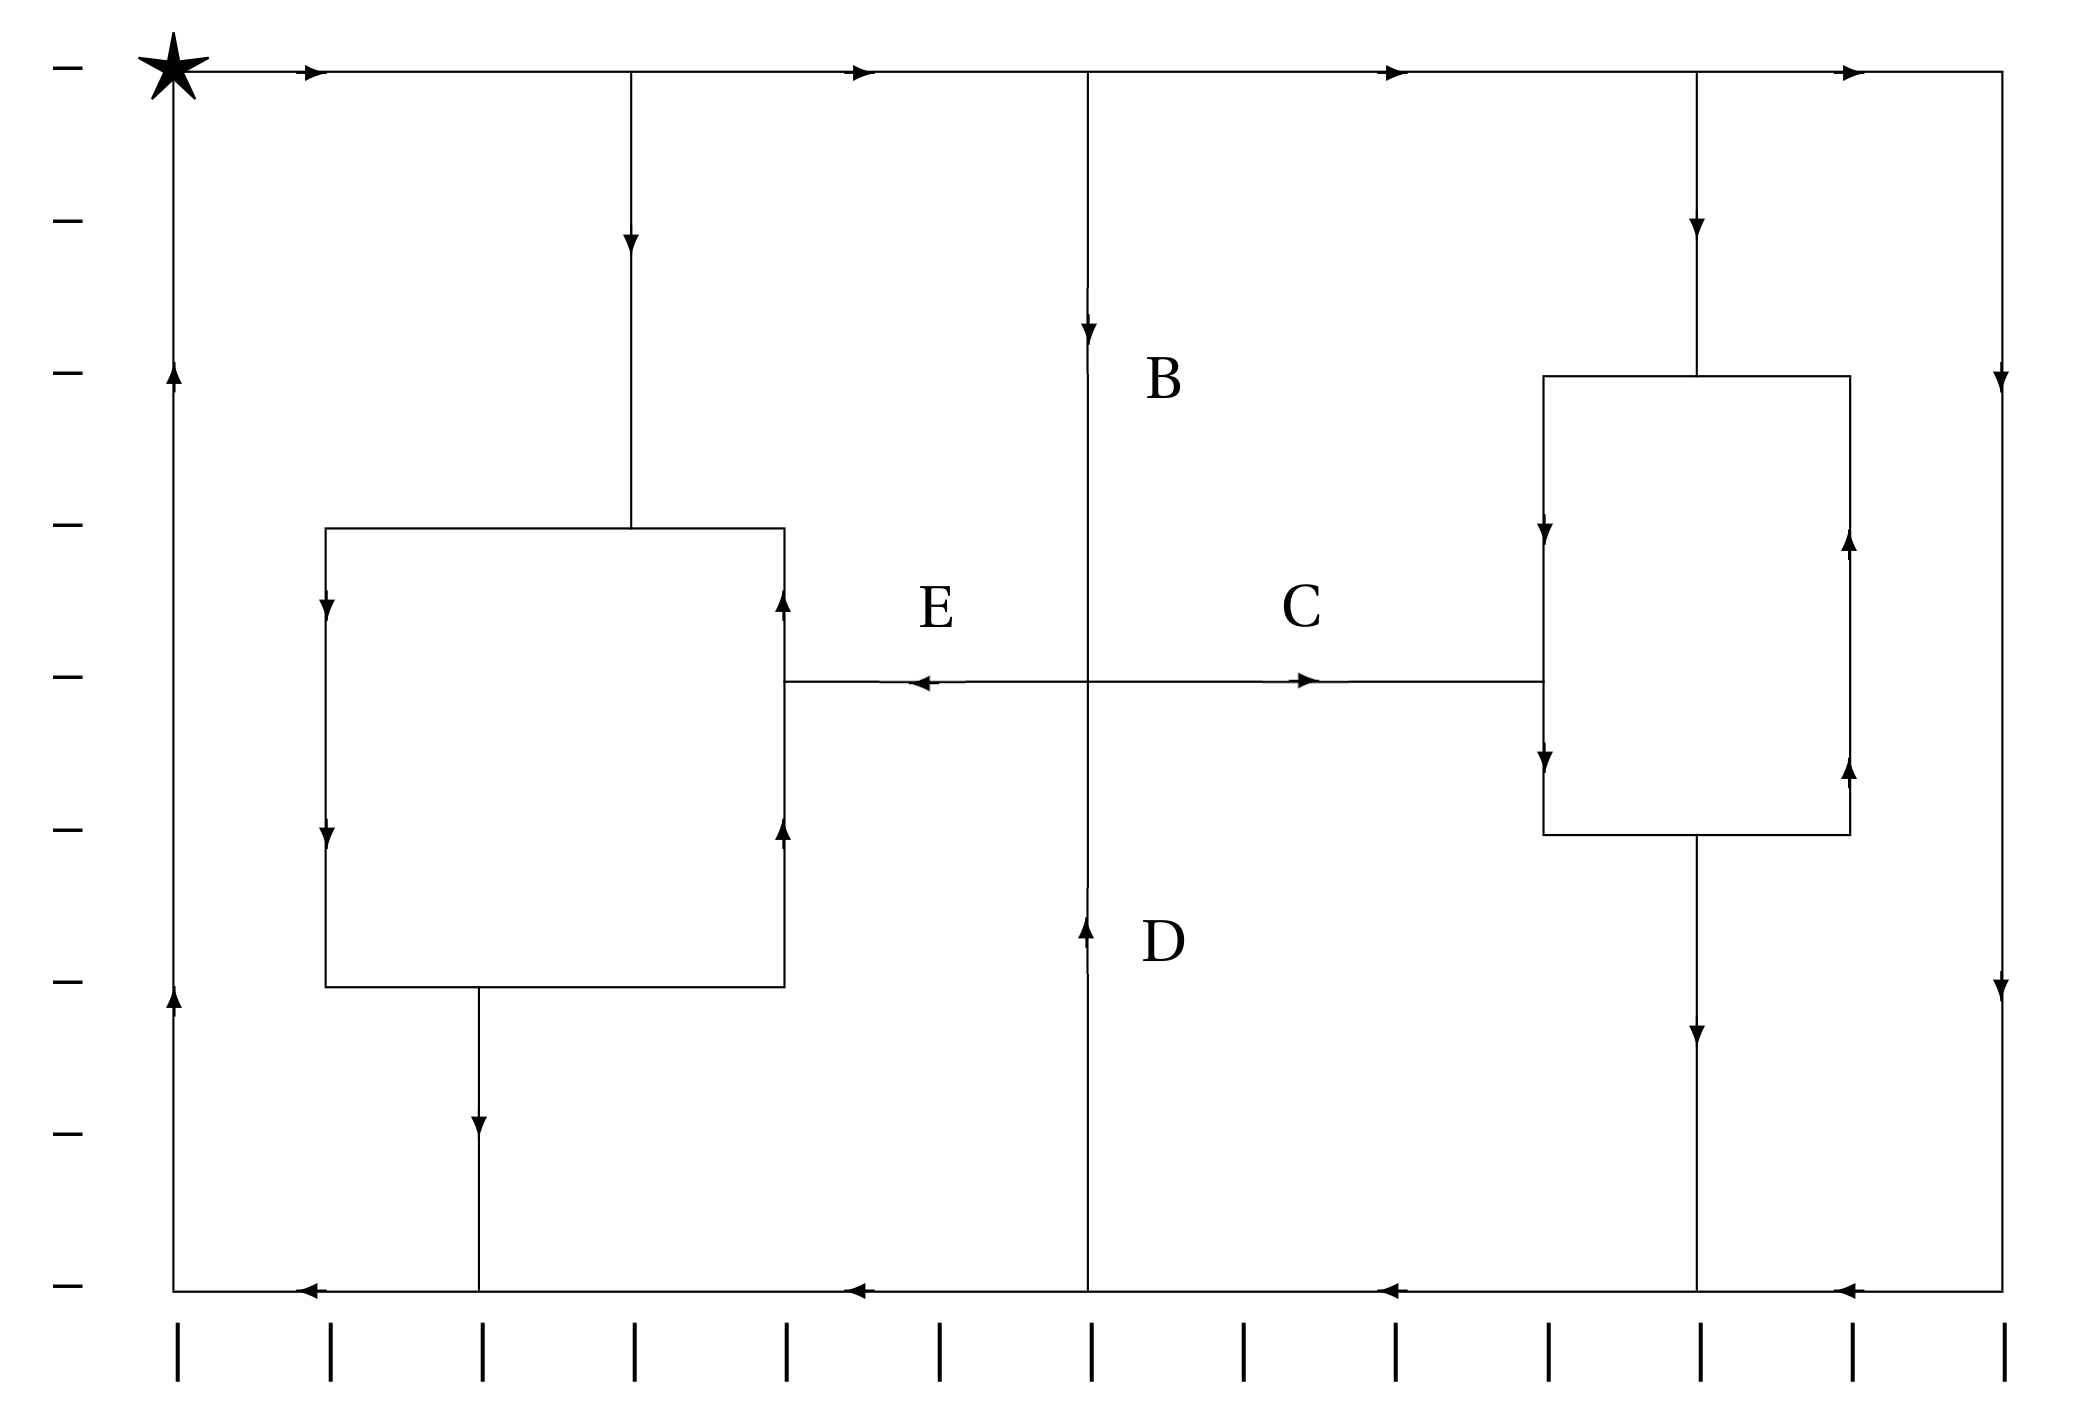
\includegraphics[width=0.5\textwidth]{images/desafio.png}\par
        \caption{representação do problema}
        \label{fig:problem}
    \end{center}
\end{figure}

Após obter esta imagem decidi-mos nomear cada vértice do problema com
uma letra maiúscula. Assim, o aspeto do desafio final utilizada é:

\begin{figure}[H]
    \begin{center}
        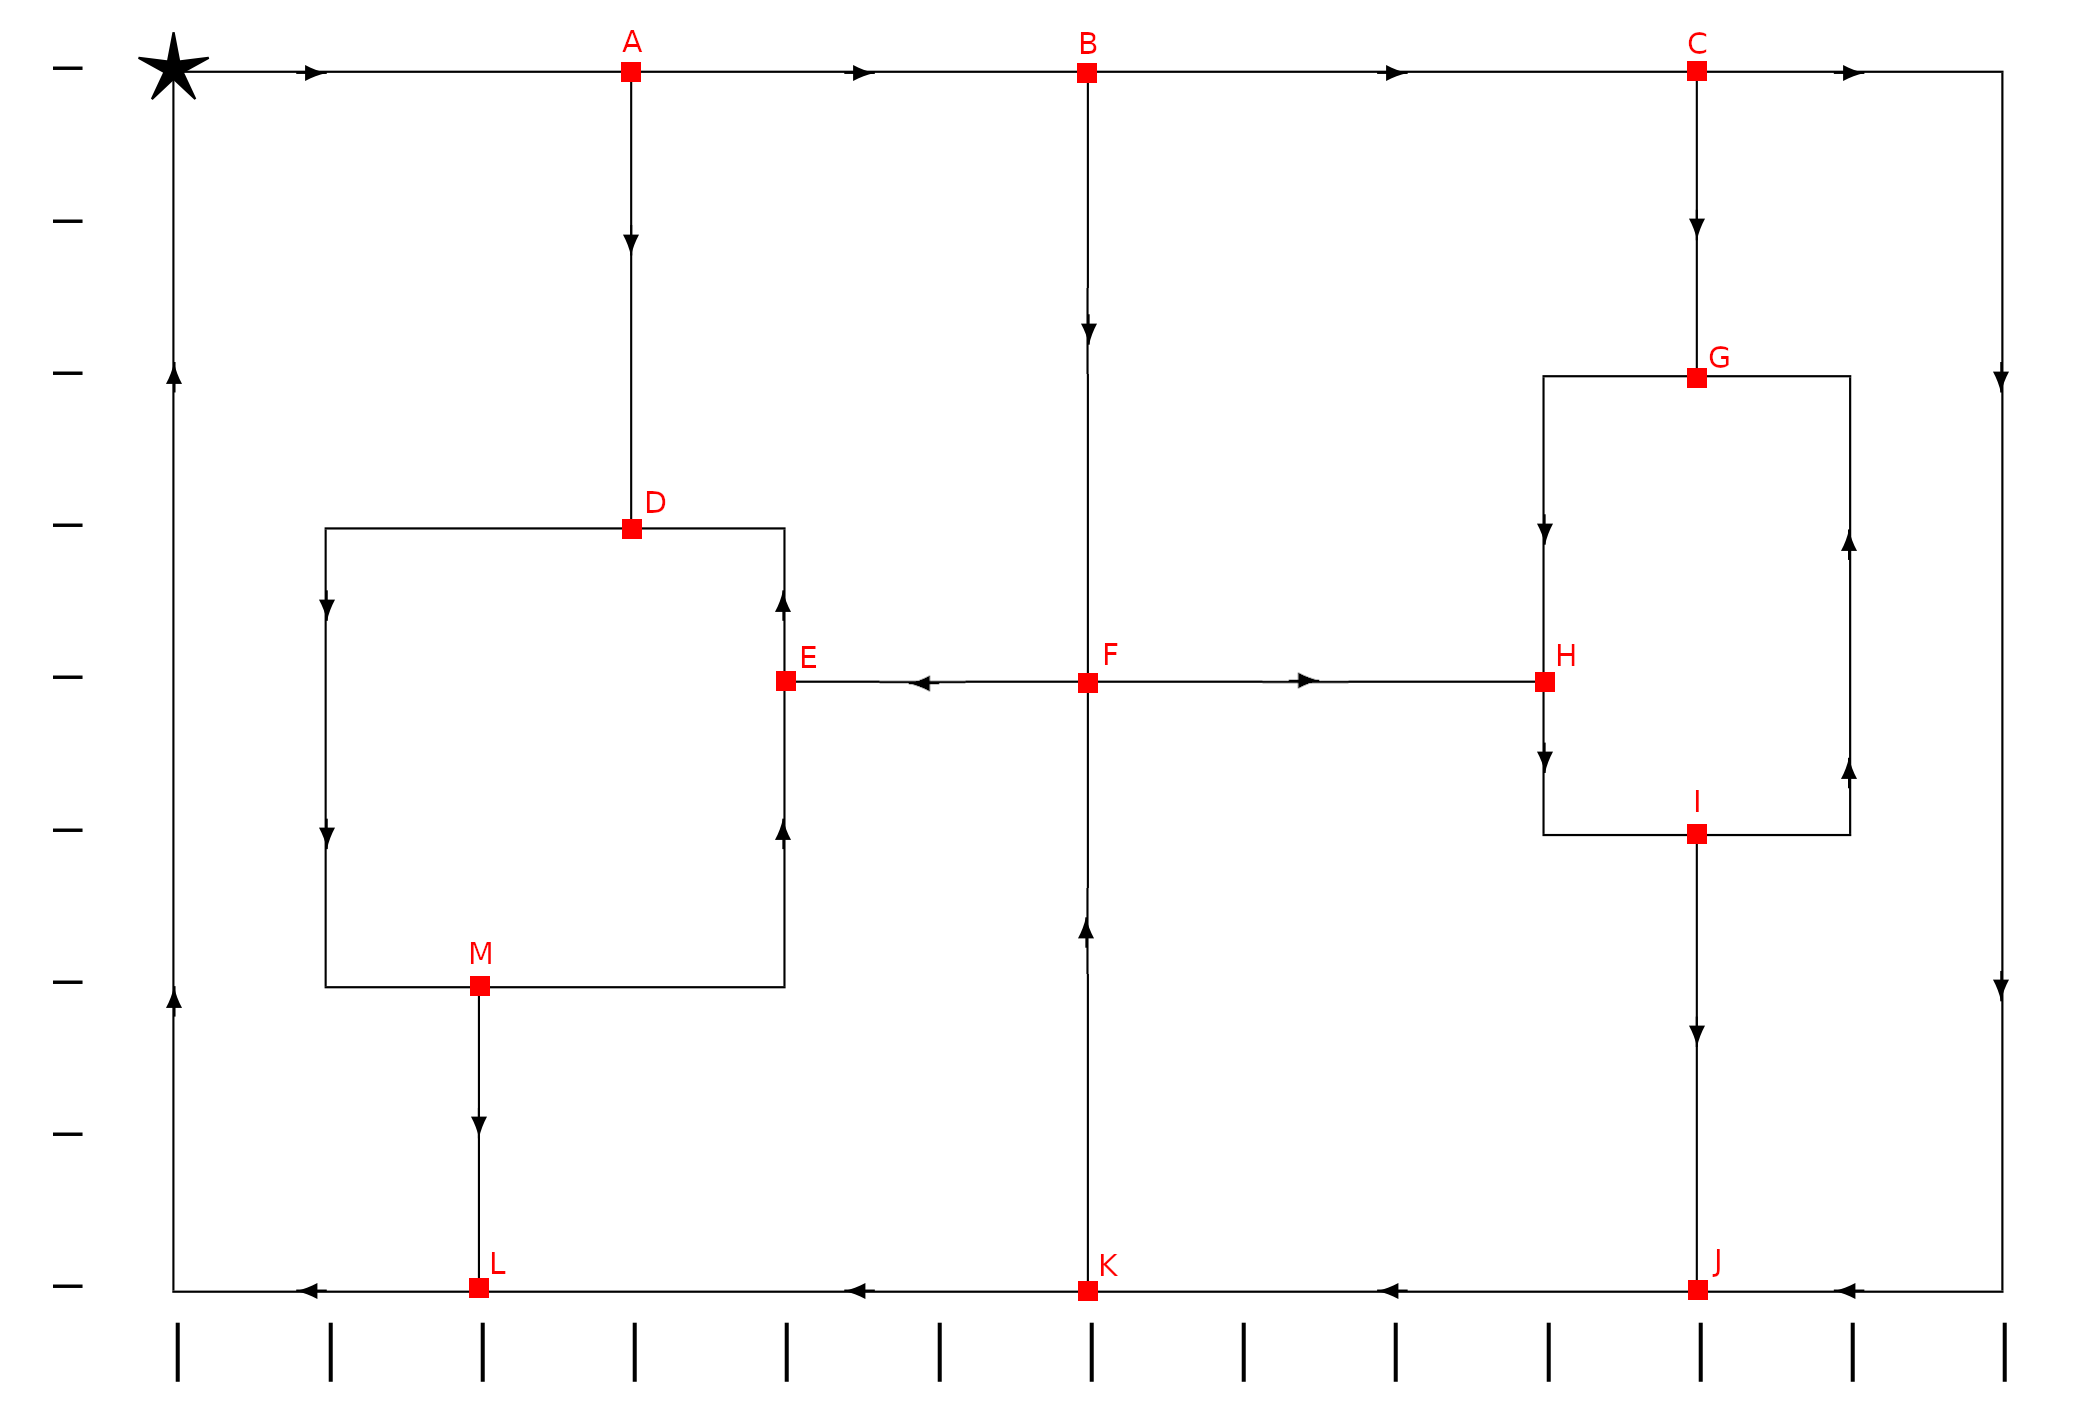
\includegraphics[width=0.9\textwidth]{images/desafioLetras.png}\par
        \caption{vértices nomeados}
        \label{fig:named}
    \end{center}
\end{figure}

\chapter{Formulação do Problema}

\section{Variáveis de decisão}
As variáveis de decisão representam o número de vezes que um dado arco
é percorrido. Por isso, é necessário que exista uma variável de decisão
por cada aresta.\\
A nomenclatura adaptada pelo grupo seguiu as seguintes regras.
As arestas têm o nome \textit{xij} em que o \textit{i} é a aresta onde
essa aresta começa e \textit{j} é o vértice onde essa aresta acaba.\\
Assim, por exemplo, a aresta \textit{xab} é a aresta que vai do 
vértice A para o vértice B.\\
Visto que cada variável representa o número de vezes que essa aresta
foi percorrida e é necessário garantir que cada aresta é visitada pelo
menos uma vez, um dos blocos de condições a que o modelo está sujeito
afirma que cada variável de decisão tem de ser maior ou igual a 1.

\section{Nodos}
Para cada nodo no mapa, a soma de todas as vezes que se entra neste
tem de ser igual à soma de todas as vezes que se sai.\\
Assim, por exemplo, para o nodo A, o número de vezes que a aresta
\textit{xla} é percorrida tem de ser igual ao número de vezes que
as arestas \textit{xad} e \textit{xab} são percorridas.
Logo, de forma a criar uma restrição para cada nodo, esta condição
pode ser formulada como:\\
\begin{multline}
xla- xad - xab = 0 \\
\end{multline}

\chapter{Texto de input}
\verbatiminput{../solution.lp}

\chapter{Ficheiro de output}
\bash[stdout]
lp_solve ../solution.lp
\END

\chapter{Interpretação do resultado}

Para facilitar a descoberta e interpretação da solução ótima alteramos 
o ponto inicial para o ponto A em vez da estrela. Esta alteração não altera 
em nada o problema do enunciado, apenas evita termos mais um ponto que pode 
ser ignorado.
Como é mostrado no ficheiro .lp, foram criadas variáveis que representam os 
nodos entre cada ponto, existindo apenas variáveis com as direções que nos 
foram propostas. Então, uma variável xAB representa o número de vezes que 
esse nodo foi percorrido.
Na nossa solução reparamos que a variável xLA é igual a 4, o que quer dizer 
que este nodo tem de ser percorrido 4 vezes e na ultima vez todos os outros 
tem de ter sido no minimo percorridos uma vez. Sabendo isto desenvolvemos a 
imagem {imagem da solução com os caminhos} com as quatro iterações da nossa 
solução ótima tendo em atenção que, por uma variável ser maior que 1, não 
significa que tenha sido percorrida as seguintes vezes só depois de ter passado 
pelo ponto inicial. Além da imagem anterior também construimos, para uma 
melhor compreensão da imagem com as iterações, a {imagem com as setas} que 
nos facilitou a vizualização de por onde precisavamos passar para realizar 
um caminho.

\begin{figure}[H]
    \begin{center}
        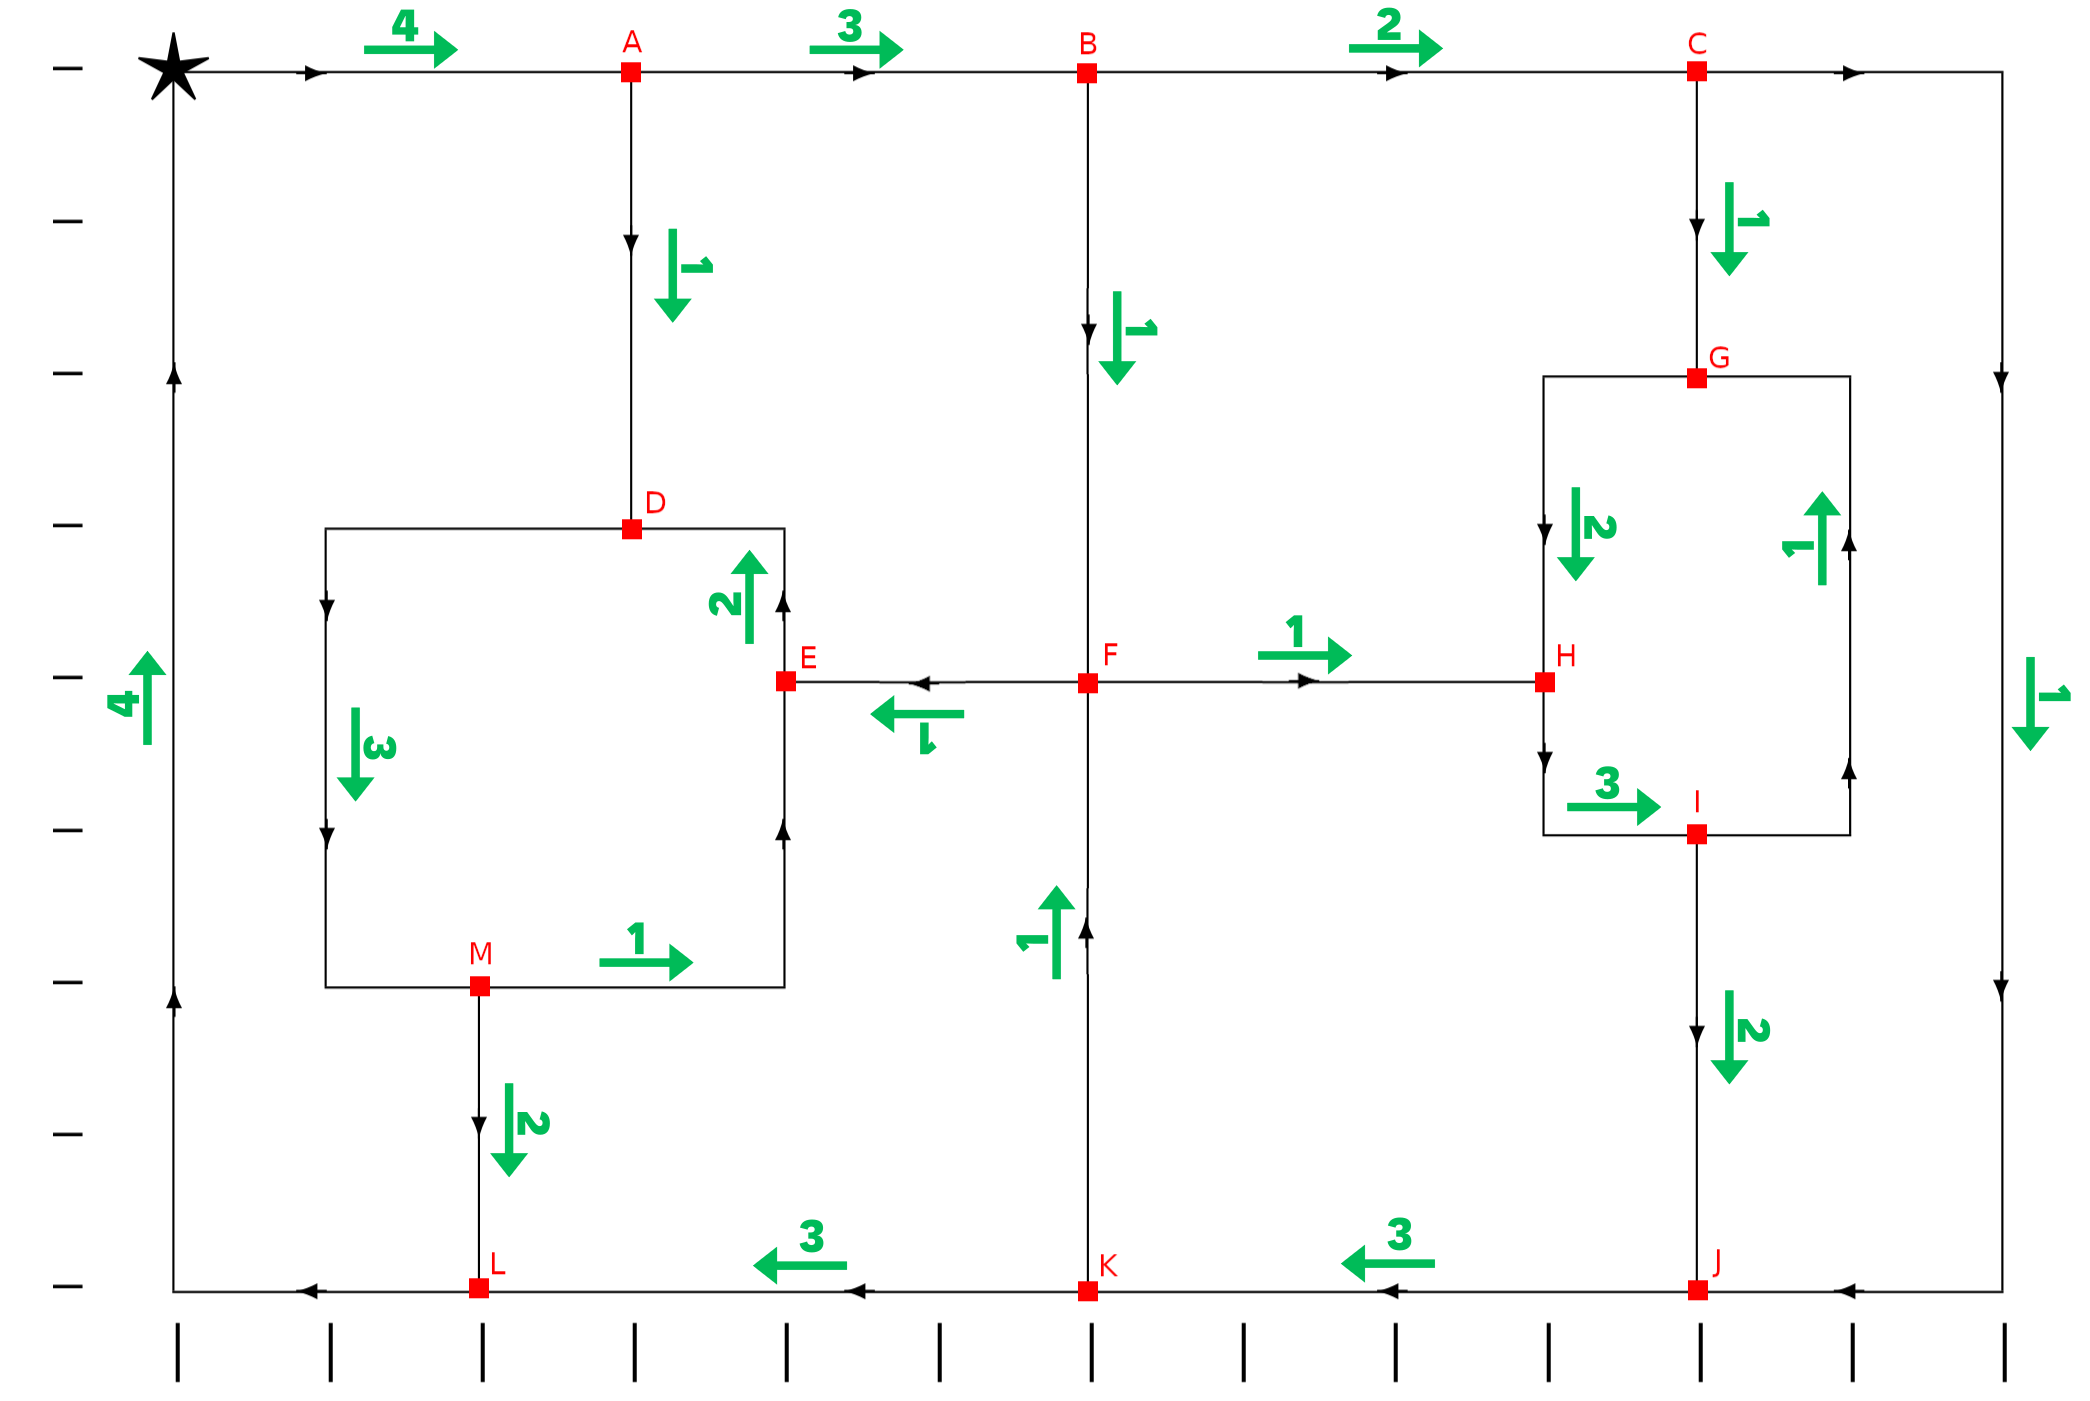
\includegraphics[width=0.9\textwidth]{images/desafioVisited.png}\par
        \caption{representação da solução}
        \label{fig:visited}
    \end{center}
\end{figure}

\begin{figure}[H]
    \begin{center}
        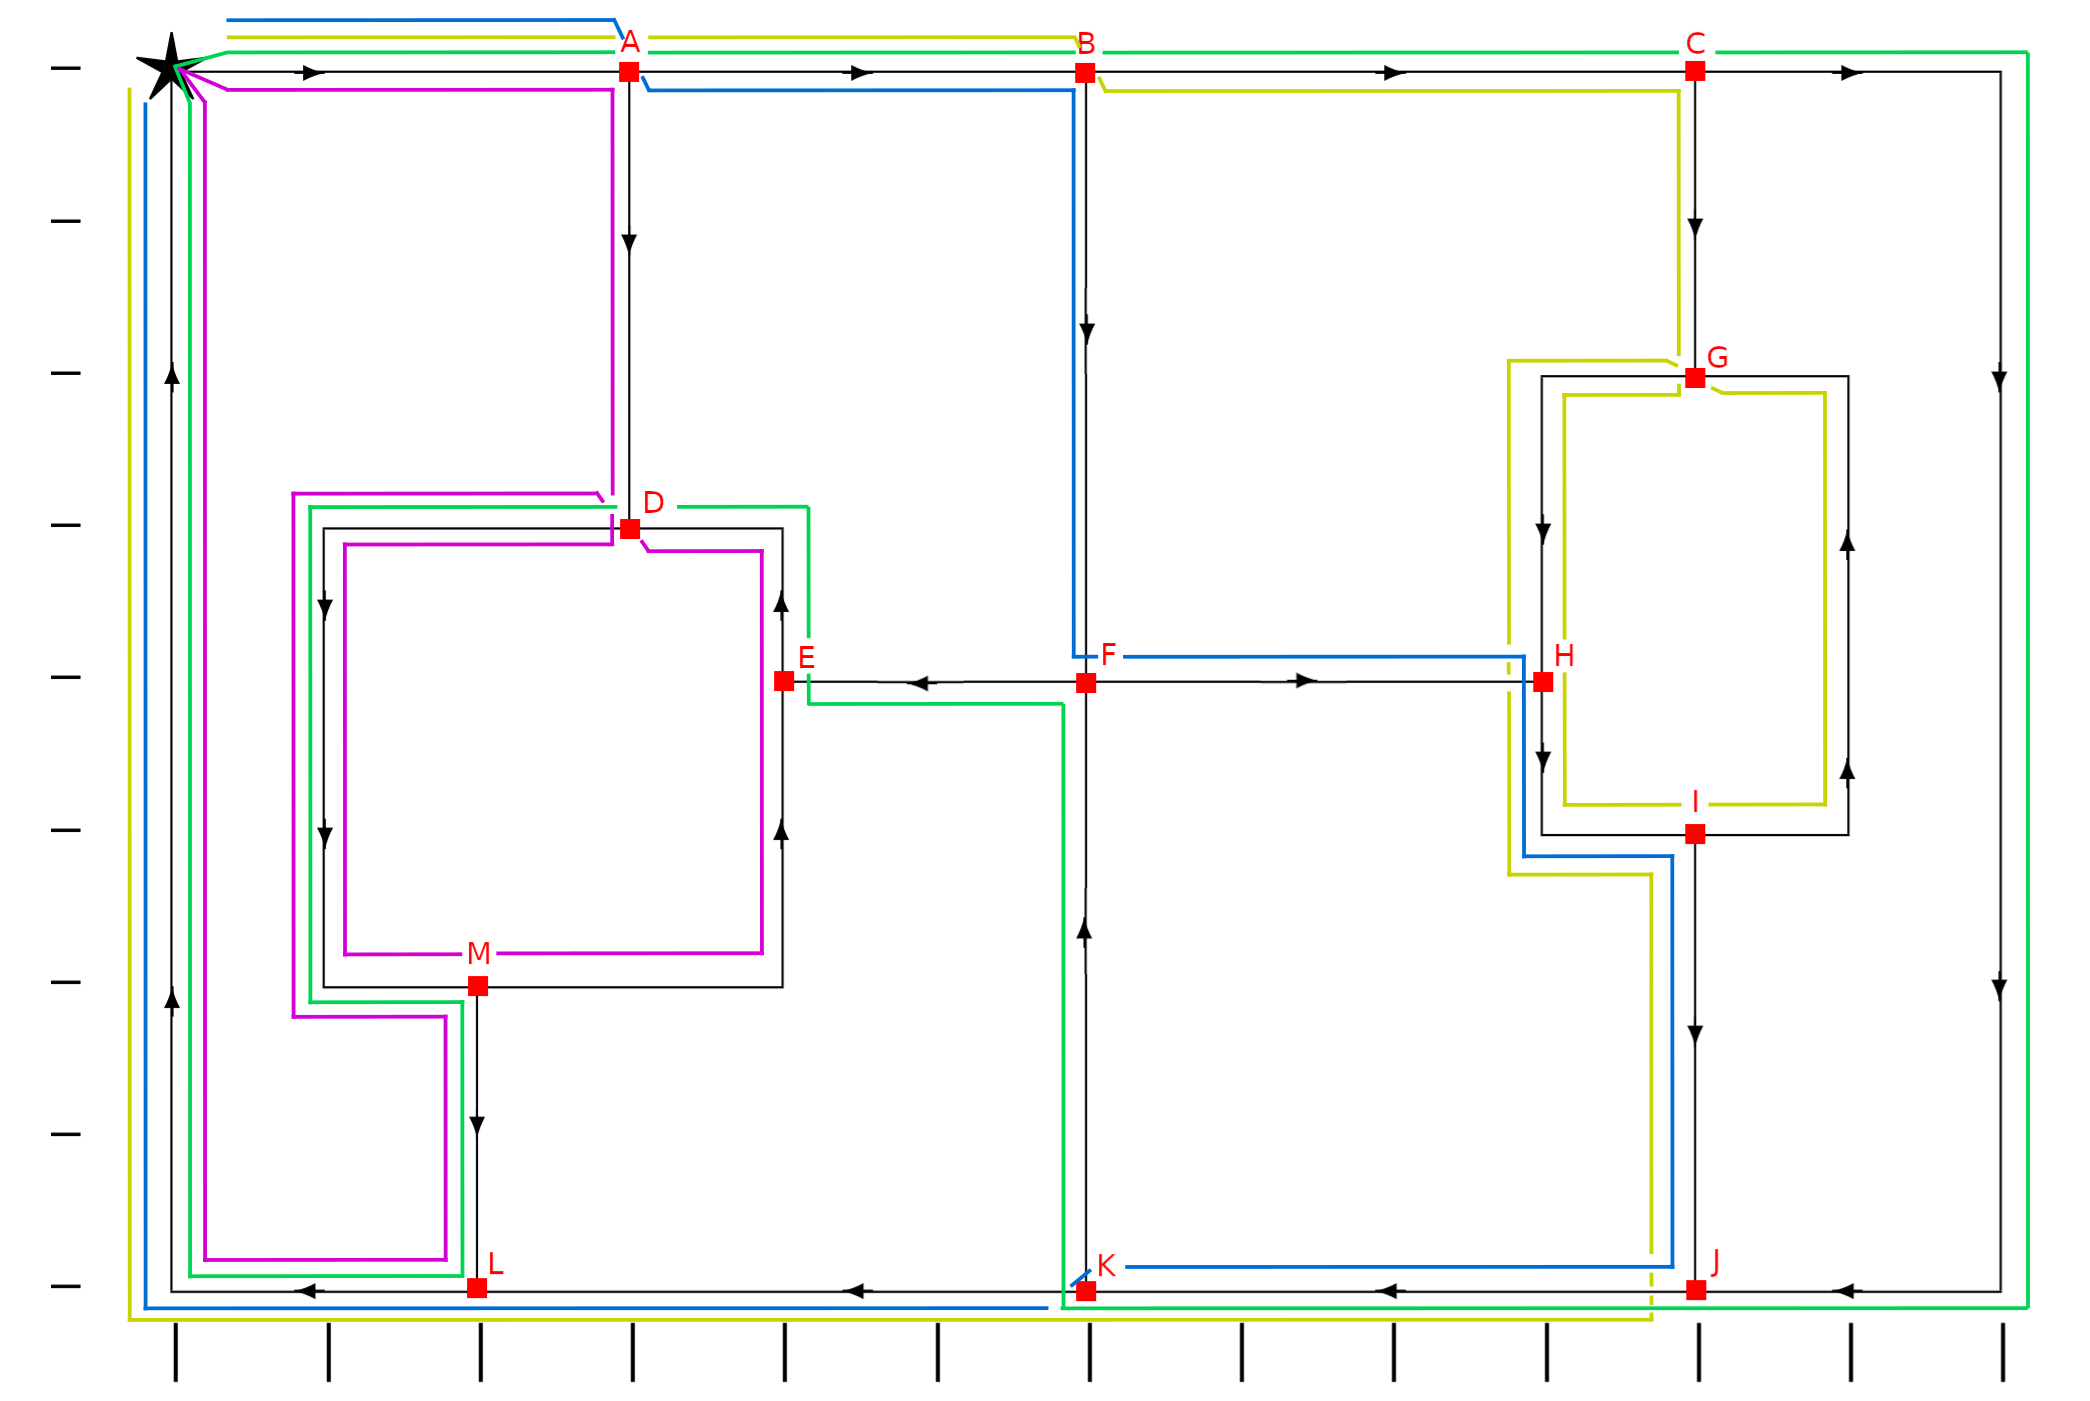
\includegraphics[width=0.9\textwidth]{images/desafioSolucao.png}\par
        \caption{representação do caminho}
        \label{fig:path}
    \end{center}
\end{figure}

\chapter{Validação do modelo}
\section{Tipo de variáveis}
As variáveis têm de ser todas do tipo inteiro pois representam o número
de vezes que essa aresta é atravessada.
De facto, após analisar os resultados obtidos, todos os resultados são
valores inteiros.\\
Visto que é necessário que cada aresta seja visitada pelo menos uma
vez, todas as variáveis têm de ter um valor maior ou igual a um, o
que de facto se verifica.

\section{Função objetivo}
O resultado da função objetivo utilizada no modelo quando o valor
das variáveis é manualmente substituindo pela solução ótima tem de 
coincidir com o resultado obtido.
Assim:

\begin{multline}
13\times xla + 3\times xab + 4\times xbc + 12\times xcj + 4\times
xjk + 4\times xkl + 4\times xkf + xfe + 2\times xed \\ + 6\times xdm +
2\times xml + 3\times xad + 4\times xbf + 3\times xfh + 2\times xcg +
3\times xgh + 2\times xhi + 3\times xij + 5\times xig + 4\times xme
\end{multline}

E substituido os vaores das variáveis de decisão:


\begin{multline}
13\times 4 + 3\times 3 + 4\times 2 + 12\times 1 + 4\times
3 + 4\times 2 + 4\times 1 + 1 + 2\times 2 + 6\times 3 +
2\times 2 + 3\times 1 \\ + 4\times 1 + 3\times 1 + 2\times 1 +
3\times 2 + 2\times 3 + 3\times 2 + 5\times 1 + 4\times 1 
= 171
\end{multline}

\section{Restrições}
\begin{multline}
A: xla - xad - xab = 0
\Rightarrow 4 - 1 - 3 = 0 
\Rightarrow 0 = 0
\end{multline}

\begin{multline}
B: xab - xbf - xbc = 0 
\Rightarrow 3 - 1 - 2 = 0
\Rightarrow 0 = 0
\end{multline}

\begin{multline}
C: xbc - xcg - xcj = 0
\Rightarrow 2 - 1 - 1 = 0
\Rightarrow 0 = 0
\end{multline}

\begin{multline}
D: xad + xed - xdm = 0
\Rightarrow 1 + 2 - 3 = 0
\Rightarrow 0 = 0
\end{multline}

\begin{multline}
E: xfe + xme - xed = 0
\Rightarrow 1 + 1 - 2 = 0
\Rightarrow 0 = 0
\end{multline}

\begin{multline}
F: xbf + xkf - xfe - xfh = 0
\Rightarrow 1 + 1 - 1 - 1 = 0
\Rightarrow 0 = 0
\end{multline}

\begin{multline}
G: xcg + xig - xgh = 0
\Rightarrow 1 + 1 - 2 = 0
\Rightarrow 0 = 0
\end{multline}

\begin{multline}
H: xgh + xfh - xhi = 0
\Rightarrow 2 + 1 - 3 = 0
\Rightarrow 0 = 0
\end{multline}

\begin{multline}
I: xhi - xig - xij = 0
\Rightarrow 3 - 1 - 2 = 0
\Rightarrow 0 = 0
\end{multline}

\begin{multline}
J: xij + xcj - xjk = 0
\Rightarrow 2 + 1 - 3 = 0
\Rightarrow 0 = 0
\end{multline}

\begin{multline}
K: xjk - xkf - xkl = 0
\Rightarrow 3 - 1 - 2 = 0
\Rightarrow 0 = 0
\end{multline}

\begin{multline}
L: xml + xkl - xla = 0
\Rightarrow 2 + 2 - 4 = 0
\Rightarrow 0 = 0
\end{multline}

\begin{multline}
M: xdm - xml - xme = 0
\Rightarrow 3 - 2 1 = 0
\Rightarrow 0 = 0
\end{multline}

\chapter{Conclusão}

\end{document}
